\documentclass[10pt,twocolumn,letterpaper]{article}
\usepackage{cvpr}
\usepackage{times}
\usepackage{latin1}
\usepackage{epsfig}
\usepackage{graphicx}
\usepackage{amsmath}
\usepackage{amssymb}
\usepackage[utf8]{inputenc} 
\usepackage[breaklinks=true,bookmarks=false]{hyperref}
\usepackage{epstopdf}
\cvprfinalcopy % *** Uncomment this line for the final submission
\def\cvprPaperID{****} % *** Enter the CVPR Paper ID here
\def\httilde{\mbox{\tt\raisebox{-.5ex}{\symbol{126}}}}

% Pages are numbered in submission mode, and unnumbered in camera-ready
%\ifcvprfinal\pagestyle{empty}\fi
\setcounter{page}{1}
\begin{document}

%%%%%%%%% TITLE
\title{Desempeño de dos métodos de clasificación: Nearest neighbour y Random forest; desde el desarrollo de un diccionario de textones y entrenaniento para cada algoritmo hasta su evaluación con la matriz de confusión.}

\author{David L. Henao\\
\begin{normalsize}
Grupo de Ingeniería Biomédica. Universidad de los Andes, Bogotá, Colombia
\end{normalsize}
\\
{\tt\small dl.henao909@uniandes.edu.co}}
% For a paper whose authors are all at the same institution,
% omit the following lines up until the closing ``}''.
% Additional authors and addresses can be added with ``\and'',
% just like the second author.
% To save space, use either the email address or home page, not both
\maketitle
%\thispagestyle{empty}

%%%%%%%%% ABSTRACT
\begin{abstract}

En el siguiente artículo se presenta la metodología desarrollada para crear dos algoritmos de clasificación supervisada (Nearest neighbour y Random forest). Estos se realizaron entrenando una base de datos con un diccionario de textones, creado a partir de un banco de filtros en 8 direcciones principales. La base de datos para entrenamiento consta de 750 imágenes de texturas clasificadas en 25 categorías. Así mismo, se evaluó cada método con una base de datos de test de 250 imágenes clasificadas en las mismas 25 categorías. Se presentan los resultados evaluativos de cada uno de los algoritmos de clasificación los cuales se obtuvieron realizando la matriz de confusión para cada método. Adicionalmente, se realizó una evaluación del tiempo que emplea cada método de clasificación una vez que se ha entrenado la base de datos. Si bien se obtuvieron resultados favorables respecto al promedio de los verdaderos positivos (68\% y 72\% para Nearest neighbour y Ramdom forest respectivamente), en todas las categorías no se presentó el mismo desempeño por lo que se proponen acciones para mejorar los algoritmos.
   
\end{abstract}

%%%%%%%%% BODY TEXT
\section{Introducción}

El propósito de la visión (tanto biológica como de máquinas), es calcular una jerarquía de interpretaciones cada vez más abstractas de las imágenes observadas (o secuencias de imágenes). Para ello, es de importancia fundamental conocer cuáles son las descripciones utilizadas en cada nivel de la interpretación. Por ejemplo, realizando una analogía con los conceptos de la física , nos preguntamos cuales son los electrones visuales, los átomos visuales y las moléculas de la percepción visual[1].
La búsqueda de las imágenes y elementos básicos de percepción no es sólo por curiosidad intelectual. Esta tiene implicaciones importantes en una serie de problemas prácticos como la reducción de dimensión, desaclopamiento de variables y el modelamiento biológico [1].

La textura se puede representar como patrones regulares repetitivos a diferentes escalas. Esta puede ser empleada para tratar el problema de clasificación agrupando regiones de la imagen con textura consistente[2]. Por su parte, los textones se refieren a las micro -estructuras fundamentales en las imágenes naturales genéricas y por lo tanto constituyen los elementos básicos en la primera percepción visual [1].

\begin{figure}[t]
\begin{center}
%\fbox{\rule{0pt}{2in} \rule{0.9\linewidth}{0pt}}
   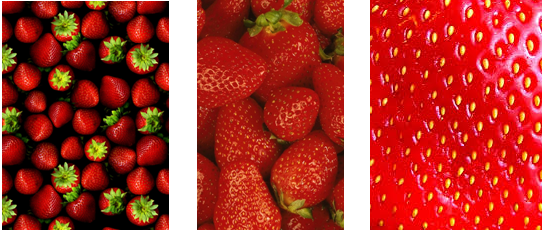
\includegraphics[width=1\linewidth]{text_esca.png}
\end{center}
   \caption{Textura en diferentes escalas.}
\label{fig:seg}
\end{figure}

Los arboles de decisión Random Forests (RF) se usan frecuentemente en muchas aplicaciones de visión computacional y aprendizaje de máquinas. Su popularidad es altamente asociada a la alta eficiencia computacional tanto para entrenamiento como para evaluación mientras se alcanzan buenos resultados [3].

Los RF poseen diferentes características que los hacen interesantes para aplicaciones de la visión computacional. Primero, son muy rápidos tanto para entrenamiento como para evaluación. Segundo, pueden ser fácilmente paralelizados. Adicionaolmente, son algoritmos multi-clases por lo que no se requiere construir diferentes clasificadores binarios para resolver problemas de este tipo[3].

Por otra parte, en los últimos años muchos investigadores se han enfocado en encontrar soluciones eficientes al problema del Nearest Neighbor, que se define como: "Dada una colección de puntos de datos y un punto P en el espacio métrico m-dimensional. Encontrar el punto de datos más cercano a P[4]. Convirtiéndose también esta, en una buena herramienta de clasificación de imágenes.

En este artículo, se muestran los resultados de clasificación obtenidos para una base de datos de imágenes durante la práctica de laboratorio. En esta práctica, se emplean los clasificadores de Nearest neighbour y Random forest a partir de entrenamiento con un diccionario de textones para clasificar dichas imágenes en 25 categorías.
%------------------------------------------------------------------------
\section{Metodología}

Para realizar la clasificación de las imágenes de prueba primero se obtuvieron dos bases de datos: una para entrenamiento y otra para test. Enseguida, se creó un diccionario de textones para efectuar con este el debido entrenamiento. Finalmente se ejecutaron los algoritmos de los clasificadores que tomaban las imágenes de prueba y las clasificaban en una de las 25 categorías existentes para posteriormente, realizar una evaluación de los resultados obtenidos para cada uno de los métodos.

\subsection{Base de datos}

La base de datos con la que se trabajó, se encuentra disponible en el servidor "guitaca" de la Universidad de los Andes (http://guainia.uniandes.edu.co/textures.zip) y consta de 1000 imágenes pertenecientes a 25 categorías.

Estas imágenes a su vez se encuentran divididas en imágenes de entrenamiento (750) e imágenes de prueba (250). Para realizar dicha división, se tomaron aleatoriamente 10 imágenes de cada categoría y se establecieron como imágenes de prueba.

Las categorías en las que están clasificadas las 25 imágenes son:

\begin{tabbing}
\hspace*{3cm} \= \hspace*{3cm} \= \hspace*{3cm} \kill
bark1 \> bark2 \> bark3 \\
wood1 \> wood2 \> wood3 \\
water \> granite \> marble \\
floor1 \> floor2 \> pebbles \\
wall \> brick1 \> brick2 \\
glass1 \> glass2 \> carpet1 \\
carpet2 \> upholstery \> wallpaper \\
fur \> knit \> corduroy \\
plaid \>  \>  \\
\end{tabbing}

Cada categoría de las mencionadas anteriormente, contiene imágenes en escala de grises con texturas en diferentes orientaciones como se muestra en la figura dos para la categoría bark1.

\begin{figure}[t]
\begin{center}
%\fbox{\rule{0pt}{2in} \rule{0.9\linewidth}{0pt}}
   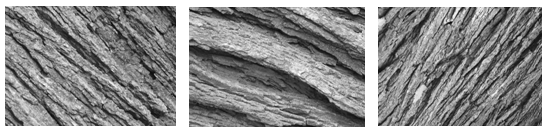
\includegraphics[width=1\linewidth]{train_tex.png}
\end{center}
   \caption{Texturas bark1 base de entrenamiento.}
\label{fig:seg}
\end{figure}

En general, en la base de datos de entrenamiento se encuentran texturas: circulares, lineales,rectangulartes, aleatorias, con un patron definido, simétricas. Todas estas desde diferentes perspectivas y orientaciones con una escala similar.

\subsection{Diccionario de textones}

Para crear el diccionario de textones se llevaron a cabo los siguientes pasos:
\begin{itemize}
\item Primero se selecionaron aleatoriamente 25 imágenes de la base de datos de entrenamiento de ( una imagen para cada categoría de 480 x 640 pixeles) y se unieron todas en unba misma imagen de 480x1600 pixeles.

\item Se creó un banco de filtros simétrico (Par con la segunda derivada Gaussiana e impar con la transformada de Hilbert) con las 8 direcciones principales que se pueden observar en la figura 3. El banco de filtros era una celda de dimensión 2x16, es decir 32 filtros.

\begin{figure}[t]
\begin{center}
%\fbox{\rule{0pt}{2in} \rule{0.9\linewidth}{0pt}}
   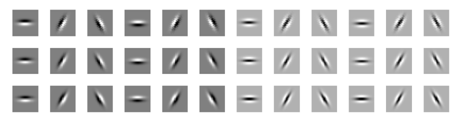
\includegraphics[width=1\linewidth]{fb.png}
\end{center}
   \caption{Texturas bark1 base de entrenamiento.}
\label{fig:seg}
\end{figure}

\item Se corrió el banco de filtros en la imagen creada en el paso 1, obteniendo así la respuesta de cada pixel de dicha imagen a cada uno de los 32 filtros. En este paso se obtuvo una respuesta de aproximadamente 7000000 de elementos.

\item Debido a las limitaciones de la memoria RAM del equipo, de dicha respuesta se tomó una muestra significativa de 6000 elementos aleatoriamente que representaran la muestra.

\item Debido a las limitaciones de la memoria RAM del equipo, de dicha respuesta se tomó una muestra significativa de 6000 elementos aleatoriamente que representaran el comportamiento de los datos.

\item Finalmente se aplicó la clasificación por kmeans a la muestra obtenida en el paso anterior para de esta manera obtener los centroides y los grupos a los que pertenece cada respuesta. Generando así nuestro diccionario de textones.

\end{itemize}
\subsection{Clasificadores}

En el caso del clasificador de Nearest neighbour, se llevaron a cabo los siguientes pasos:

\begin{itemize}
\item Se realizó el entrenamiento del algoritmo asignando los textones del diccionario a cada una de las 750 imágenes de prueba. Al final, se hallaron los histogramas correspondientes a dicha asignación.

\item Se asignaron los textones del diccionario a cada una de las 250 imágenes de test. Al final, se halló el histograma para cada una de dichas asignaciones obteniendo una celda con 250 histogramas cada uno con 50 valores.

\item Se realizó una comparación entre el histograma de una imágen de prueba con cada uno de los 750 histogramas de las imágenes de entrenamiento. Así, se obtuvo un vector de datos de 750x1 con los valores de similitud entre cada comparación teniendo como parámetro la distancia "chi square". Este vector contiene números entre 0 y 1, representando 1 una distancia muy grande (poca similitud entre histogramas) y 0 distancias muy pequeñas (mayor similitud entre histogramas).

\item Se halló el valor mínimo de este vector (pues se requiere una mayor similitud entre histogramas) y la posición asociada a dicho mínimo. Esta posición se busca en las imágenes de entrenamiento y nos indica la categoría a la que pertenece la imagen de test.

\item Se repiten los pasos 3 y 4 para las 249 imágenes restantes y una vez que se tienen todas las posiciones asociadas a los mínimos, se realiza un recorrido por las posiciones de las imágenes de entrenamiento extrayendo el nombre de la categoría de cada imagen de test.

\end{itemize}

Finalmente, para el clasificador de Random Forest está fue la metodología: 

\begin{itemize}

\item Se realiza el mismo proceso de los pasos 1 y 2 del clasificador Nearest neighbour (ver sección anterior) hallando los histogramas asociados.

\item Se crea un vector con las etiquetas de cada categoría para las imágenes de entrenamiento y se define el número de arboles que se requieren.

\item Se entrena el bosque de decisión empleando la función TreeBagger disponible en las librerías de Matlab, teniendo como parámetros de entrada el número de arboles, los histogramas y las etiquetas de los datos de entrenamiento.

\item Finalmente, se emplea el bosque del punto anterior ingresando en el cada una de las 250 imágenes de test. Obteniendo como respuesta la categoría a la que pertenece cada una de estas imágenes.

\end{itemize}


%------------------------------------------------------------------------
\section{Resultados}

Para evaluar y comparar el desempeño de los métodos de clasificación realizados en el presente artículo, se calculó la matriz de confusión de cada uno de ellos. El desempeño ideal para ambos métodos debía ser obtener una matriz con una diagonal de 10 lo que nos indicaba que no existían falsos positivos o falsos negativos sino que la clasificación de cada imagen fue correcta deacuerdo a la categoría real asignada.

\subsection{ Matriz de confusión Nearest neighbour y Random forest}

Se realizó la matriz de confusión con las etiquetas de datos reales para los métodos de Nearest neighbour y Random forest los resultados se pueden apreciar en las figuras 4 y 5 respectivamente.

\begin{figure}[t]
\begin{center}
%\fbox{\rule{0pt}{2in} \rule{0.9\linewidth}{0pt}}
   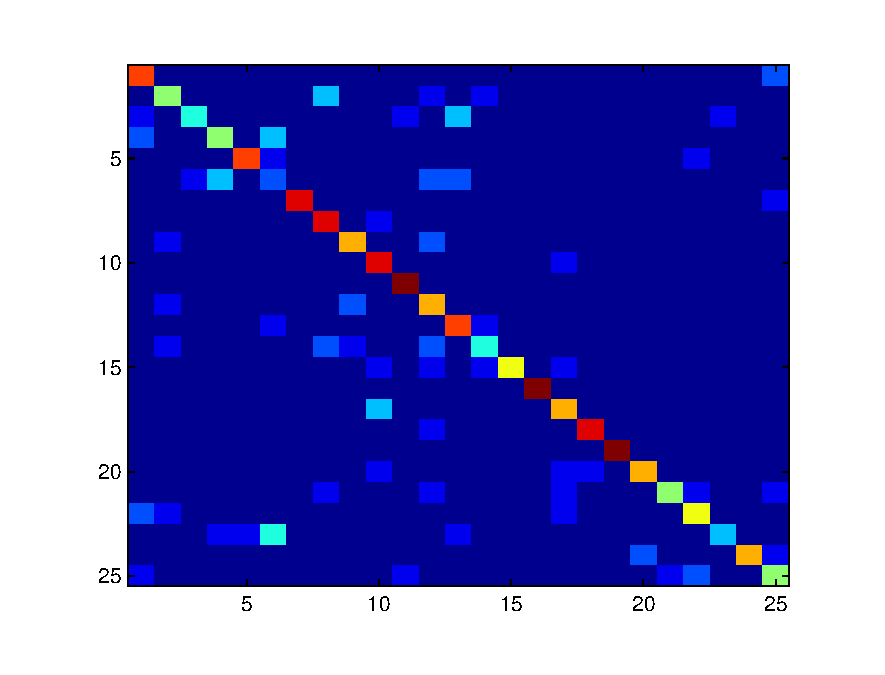
\includegraphics[width=1\linewidth]{con_chi.eps}
\end{center}
   \caption{Matriz de confusión, clasificación por Nearest neighbour}
\label{fig:seg}
\end{figure}


\begin{figure}[t]
\begin{center}
%\fbox{\rule{0pt}{2in} \rule{0.9\linewidth}{0pt}}
   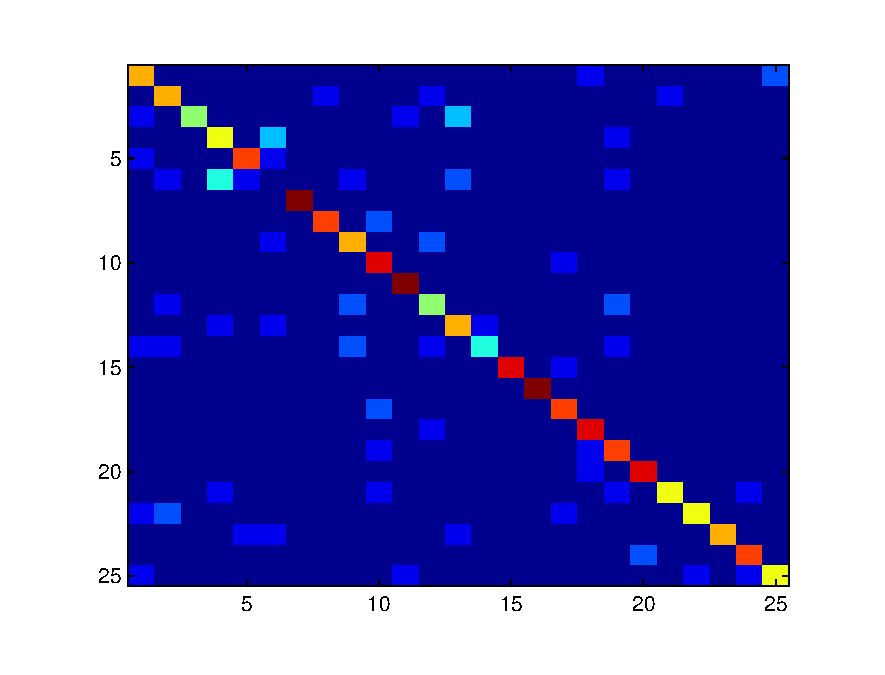
\includegraphics[width=1\linewidth]{con_arb.eps}
\end{center}
   \caption{Matriz de confusión, clasificación por Random forest.}
\label{fig:seg}
\end{figure}

La diagonal de la matriz de confusión obtenida para el método de clasificación de Nearest neighbour fue:\\

Dn = [8,5,4,5,8,2,9,9,7,9,10,7,8,4,6,10,7,9,10,7,5,6,3,7,5].\\

y el promedio de ésta fue de 6.8 por lo que en términos generales el algoritmo tuvo un desempeño del 68\%.

La diagonal de la matriz de confusión obtenida para el método de clasificación de Random forest fue:\\

Df = [7,7,5,6,8,0,10,8,7,9,10,5,7,4,9,10,8,9,8,9,6,6,7,8,6].\\

y el promedio de ésta fue de 7.16 por lo que en términos generales el algoritmo tuvo un desempeño del 71.6\%.


\subsection{Parámetros y tiempo de clasificación de cada algoritmo}

La selección de los parámetros para ambos algoritmos de clasificación se describe a continuación:\\

Nearest neighbour\\

Para seleccionar el tipo de filtros a crear en el banco de filtros, se analizaron las texturas de la base de datos de entrenamiento. Se observó que la mayoría de las imágenes de dicha base de datos presentaba texturas lineales por lo que se crearon este tipo de filtros y no se tuvieron en cuenta los filtros circulares.

Ahora bien, el número de clusters seleccionados fue de 50. Esto debido a que se quieren agrupar las 32 respuestas de cada pixel a los filtros y no agrupar las respuestas similares en un mismo clusters por lo que se selecciona un número mayor a 32 pero que no sobre especialice el algoritmo.

Respecto a los árboles de decisión\\ 

Para seleccionar el número de árboles en el bosque, se tuvo en cuenta la gráfica presentada en la figura 6. En esta gráfica se obtiene en el momento de entrenar el bosque y nos muestra como se minimiza el error con el incremento del número de árboles. Ahora bien, a pesar de que aumento del número de árboles  minimiza dicho error, este converge hasta el punto en que nuestro algoritmo se comienza a sobre especializar. Este es un efecto indeseado en el sentido que se quiere que el método pueda clasificar diferentes texturas similares y no solo la textura de clasificación. Observando la gráfica, el número de árboles seleccionado fue de 500.

El tiempo de clasificación para cada algoritmo, incluyendo el tiempo de entrenamiento con las 750 imágenes de la base de datos fue:

\begin{tabbing}
\hspace*{3cm} \= \hspace*{3cm}\kill

Nombre \> tiempo (s) \\
Nearest neighbour \> 1098.58 \\
Random forest \> 1641.60 \\

\end{tabbing}


Chi = 1098.58 s
Arb = 1641.60 s


\begin{figure}[t]
\begin{center}
%\fbox{\rule{0pt}{2in} \rule{0.9\linewidth}{0pt}}
   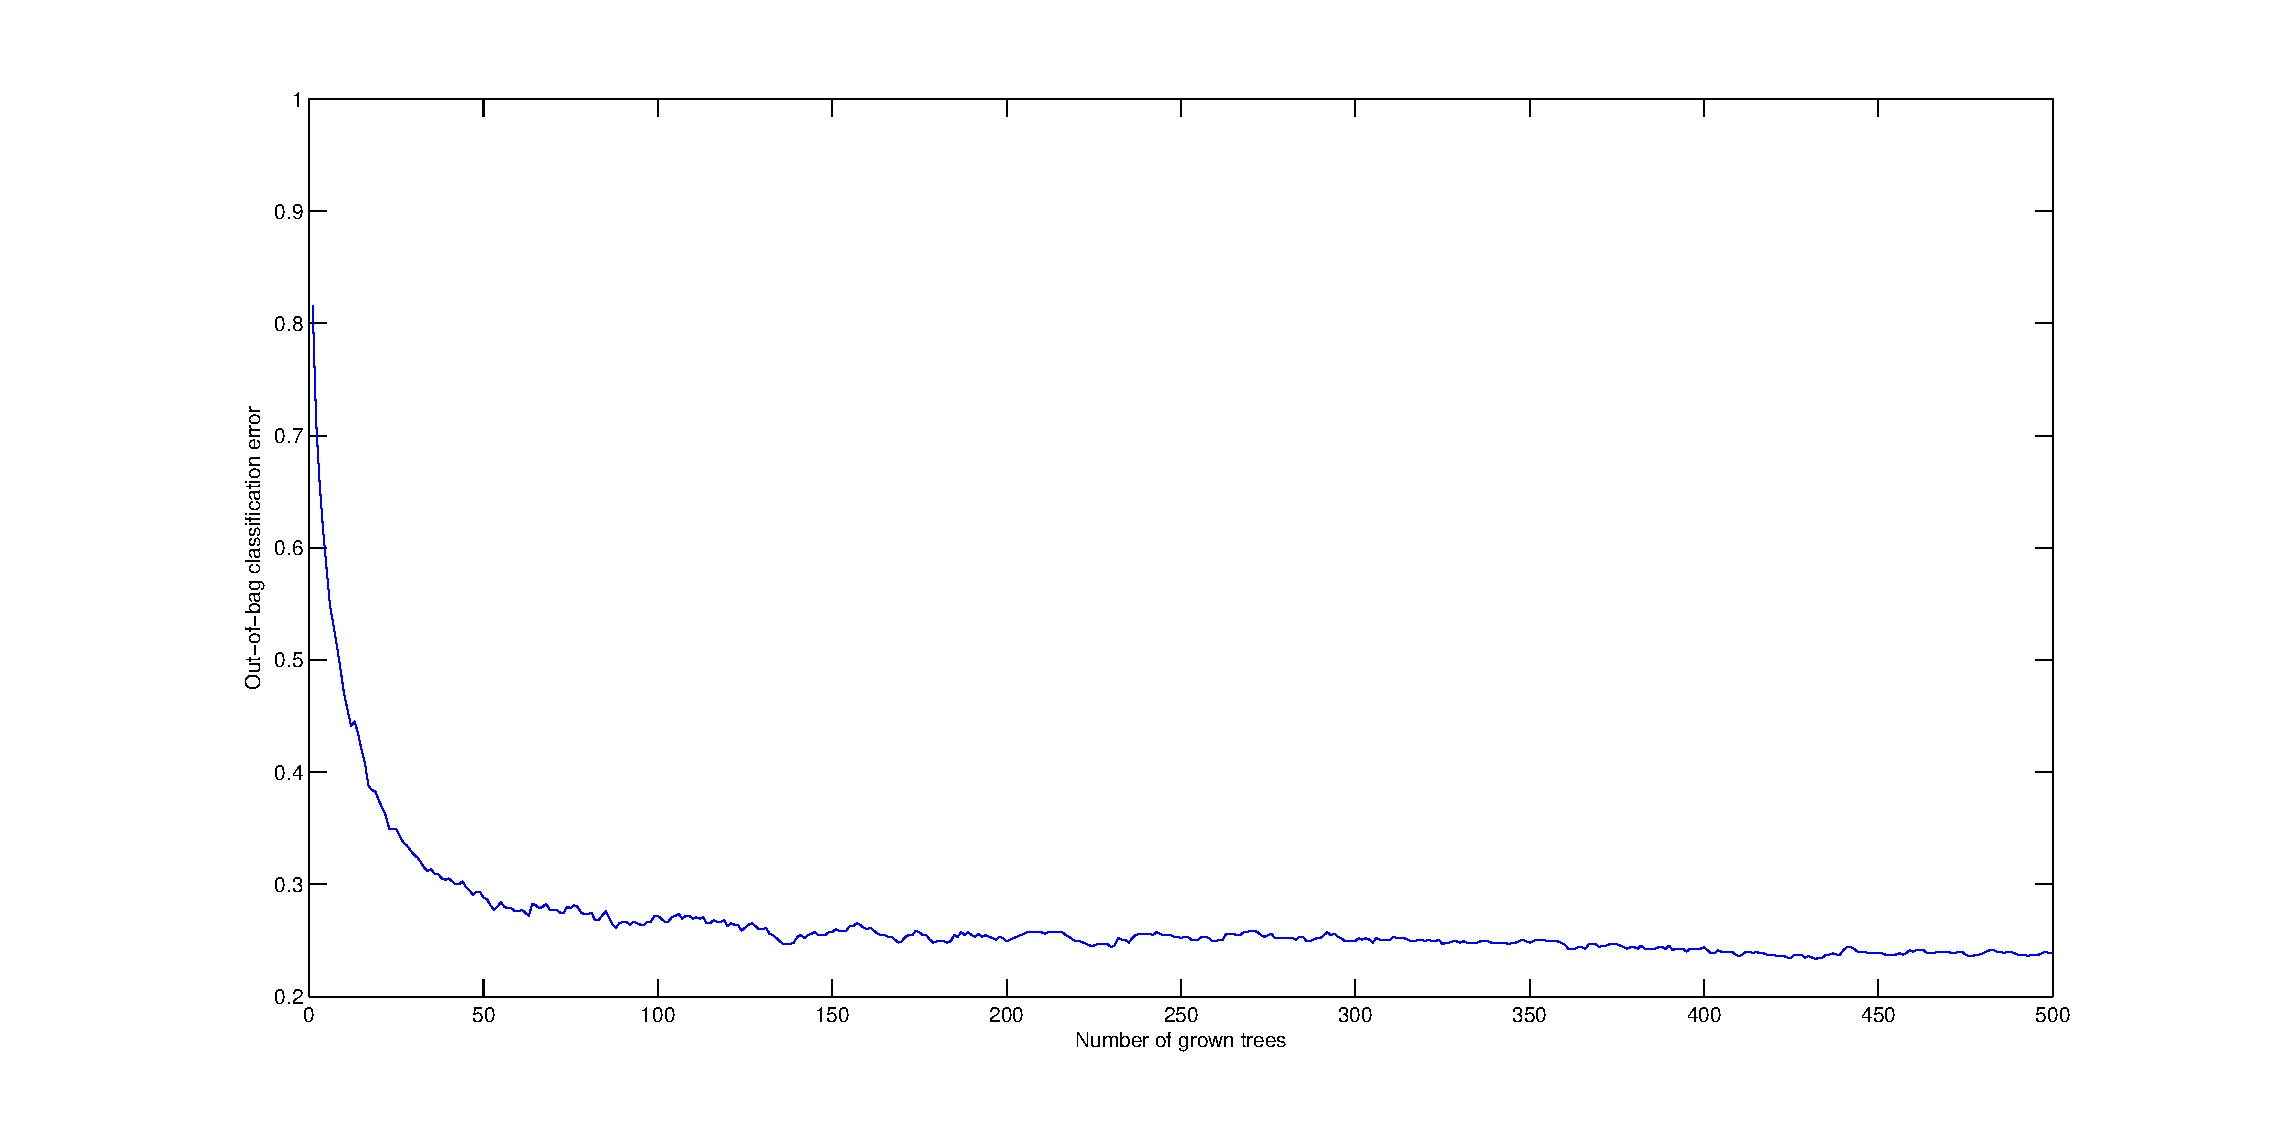
\includegraphics[width=1\linewidth]{arbolerror.eps}
\end{center}
   \caption{Error vs número de arboles en el bosque de decisión}
\label{fig:seg}
\end{figure}

%------------------------------------------------------------------------
\section{Discusión}

Respecto al mejor clasificador\\

El mejor clasificador, respecto al desempeño definitivamente fue Random forest. A pesar de que con el clasificador de Nearest neighbour se realizó la clasificación de las 250 imágenes en 543.02 segundos menos (9 minutos), el resultado de la clasificación acertada disminuyó significativamente. Por otro lado, este tiempo adicional que empleó el arbol de decisión se puede reducir notoriamente con un menor número de arboles de decisiones. Todo esto es posible sin incrementar el error seleccionando un parámetro adecuado para k.

Respecto a las limitaciones del método y la base de datos\\

Ambos métodos parten de un diccionario de textones creado a partir de kmeans. Es bien conocido que Kmeans tiende a formar grupos esféricos alrededor de los centroides de inicialización por lo que en el momento de realizar clasificación, para textones muy separados, no suele tener el mejor desempeño en el sentido que tiene en cuenta la distancia euclídea entre los textones y
sus centroides.
Por otro lado, dichos grupos suelen ser del mismo tamaño por lo que para texturas con regiones a diferentes escalas, la segmentación no suele ser la más efectiva y depende de la inicialización de los centroides que el algoritmo converja a mínimos locales.

Por otro lado, las principales limitaciones del método de Randomforest, radican en que se sobreajusta en grupos de datos ruidosos. Esto lo pudimos observar en la categoría 6 donde se presentó la peor clasificación producto del tipo de imagen. Por otro lado, para los datos que incluyen categorías con diferente número de niveles, el método de Randomforests se parcializa a favor de atributos con más niveles. Esto lo podemos observar en las categorías 15 a 20 que eran las que tenían texturas más complejas respecto a su composición (y podían responder a diferentes filtros a la vez). 
En cuanto a las limitaciones de la base de datos empleada se tiene que: es muy pequeña por lo que no nos da un entrenamiento confiable de nuestro método y las imágenes de la base de datos fueron tomadas con las condiciones de iluminación, distancia, foco adecuado para los métodos. En otras palabras fueron preparadas para realizar los métodos descritos en este reporte por lo que no se aproximan a la clasificación de imágenes que a largo plazo queremos realizar que son las imágenes de la cotidianidad y es lógico que nos den desempeños superiores al 70\%.
Para mejorar ambos métodos se propone realizar un preprocesamiento de la imagen para filtrar los datos ruidosos o bien un procesamiento que evite el sobreajuste hacia datos de ruido como una distribución de probabilidad ignorando estas clases. Además, se pudo observar que cambiando el diccionario de textones se obtenían diferentes valores de desempeño para ambos métodos (midiendo este como el promedio de cada matriz de confusión). Se puede crear un diccionario de textones que se ajuste de una mejor manera a las texturas que se desean entrenar, por ejemplo incluir un filtro circular en el banco de filtros y aplicar un método diferente al seleccionar la sub muestra de todas las imágenes para tener la certeza de que se generen las respuestas específicas para cada dirección deseada.
Para  solucionar el problema del diferente número de niveles entre categorías en Randomforest,  se propone implementar con anterioridad un método como el de permutaciones parciales. Adicionalmente se puede realizar una mejor elección de K, realizar un estudio más amplio en que halle el punto óptimo en el que se reduce el efecto del ruido en la clasificación sin crear límites no deseados entre clases similares. Pues a pesar de que en  500 árboles se encuentran los valores mínimos de ruidos puede que la diferencia con 100 árboles no sea la más significativa pero el tiempo de cómputo si es 5 veces mayor.
Respecto al método del vecino más cercano, se puede mejorar ponderando la contribución de cada vecino de acuerdo a la distancia entre él y el centroide, dando un mayor peso a los vecinos más cercanos y empleando un método más robusto/ adecuado para la comparación de los histogramas como lo es el de intersección en vez de chisq.

\vspace{7 cm}

%------------------------------------------------------------------------
\section{Referencias}

$[1]$
S.-C. Zhu, C. Guo, Y. Wang, and Z. Xu, “What are Textons?,” Int J Comput Vision, vol. 62, no. 1–2, pp. 121–143, Apr. 2005.\\

\vspace{0.15 cm}
$[2]$
P.A. Arbelaez, "Representación". Visión Artificial, Tema 6. Universidad de los Andes, Bogotá. Febrero 2015.\\

\vspace{0.15 cm}
$[3]$
A. Saffari, C. Leistner, J. Santner, M. Godec, and H. Bischof, “On-line Random Forests,” in 2009 IEEE 12th International Conference on Computer Vision Workshops (ICCV Workshops), 2009, pp. 1393–1400.\\

\vspace{0.15 cm}
$[4]$
K. Beyer, J. Goldstein, R. Ramakrishnan, and U. Shaft, “When Is ‘Nearest Neighbor’ Meaningful?,” in In Int. Conf. on Database Theory, 1999, pp. 217–235.\\

\end{document}
